\chapter{Конструкторская часть}

В данном разделе представлены этапы проектирования баз данных.


\section{Проектирование базы данных}

В соответствии с таблицей \ref*{tbl:categories} база данных должна содержать следующие таблицы:


\begin{table}[H]
	\centering
	\caption{Company (таблица компаний)}
	\label{tbl:companies}
	\resizebox{\textwidth}{!}{%
		\begin{tabular}{|c|c|c|}
			\hline
			\textbf{Атрибут} & \textbf{Тип} & \textbf{Значение}  \\ \hline
			id                     & Целое число             & Идентификатор, PK   \\ \hline
			name                     & Строка              & Название                 \\ \hline
			logo                     & Строка             & Путь к логотипу                   \\ \hline
			description                			& Строка             & Описание                       \\ \hline
			ticker                			& Строка             & Тикер                       \\ \hline
			indicators\textunderscore id                			& Целое число             & Идентификатор показателей для соответствующей компании, FK                       \\ \hline
		\end{tabular}
	}
\end{table}



\begin{table}[H]
	\centering
	\caption{Forecast (таблица прогнозов)}
	\label{tbl:forecasts}
	\resizebox{\textwidth}{!}{%
		\begin{tabular}{|c|c|c|}
			\hline
			\textbf{Атрибут} & \textbf{Тип} & \textbf{Значение}  \\ \hline
			id                     & Целое число             & Идентификатор, PK   \\ \hline
			invest\textunderscore house                     & Строка              & Инвест-дом                 \\ \hline
			date\textunderscore publishing                     & Дата             & Дата публикации                   \\ \hline
			date\textunderscore end                			& Дата             & Дата окончания                       \\ \hline
			date\textunderscore update                			& Дата             & Дата обновления                       \\ \hline
			goal\textunderscore price                			& Вещественное число             & Целевая цена                       \\ \hline
			forecast                			& Строка             & Прогноз                       \\ \hline
			description                			& Строка             & Описание                       \\ \hline
			company\textunderscore id                			& Целое число             & Идентификатор компании для соответствующего прогноза, FK                       \\ \hline
		\end{tabular}
	}
\end{table}


\begin{table}[H]
	\centering
	\caption{Indicators (таблица финансовых показателей)}
	\label{tbl:indicators}
	\resizebox{\textwidth}{!}{%
		\begin{tabular}{|c|c|c|}
			\hline
			\textbf{Атрибут} & \textbf{Тип} & \textbf{Значение}  \\ \hline
			id                     & Целое число             & Идентификатор, PK   \\ \hline
			price                     & Вещественное число              & Цена                 \\ \hline
			market\textunderscore cap                     & Вещественное число             & Капитализация                   \\ \hline
			income                			& Целое число             & Прибыль от выручки выраженная в процентах                       \\ \hline
			revenue                			& Вещественное число             & Выручка                       \\ \hline
		\end{tabular}
	}
\end{table}

\begin{table}[H]
	\centering
	\caption{News (таблица новостей)}
	\label{tbl:news}
	\resizebox{\textwidth}{!}{%
		\begin{tabular}{|c|c|c|}
			\hline
			\textbf{Атрибут} & \textbf{Тип} & \textbf{Значение}  \\ \hline
			id                     & Целое число             & Идентификатор, PK   \\ \hline
			title                     & Строка              & Заголовок                 \\ \hline
			date\textunderscore publishing                			& Дата             & Дата публикации                       \\ \hline
			content                			& Строка             & Наполнение                       \\ \hline
			url                			& Строка              & Ссылка на источник                       \\ \hline
			author                			& Строка              & Автор новости                       \\ \hline
			company\textunderscore id                			& Целое число             & Идентификатор компании для соответствующей новости, FK                       \\ \hline
		\end{tabular}
	}
\end{table}


\begin{table}[H]
	\centering
	\caption{User (таблица пользователей)}
	\label{tbl:user}
	\resizebox{\textwidth}{!}{%
		\begin{tabular}{|c|c|c|}
			\hline
			\textbf{Атрибут} & \textbf{Тип} & \textbf{Значение}  \\ \hline
			id                     & Целое число             & Идентификатор, PK   \\ \hline
			username                     & Строка              & Никнейм пользователя                 \\ \hline
			password                			& Строка             & Пароль пользователя, хранящийся в шифрованном виде                       \\ \hline
			email                			& Строка             & Электронная почта                        \\ \hline
			name                			& Строка              & Имя                       \\ \hline
			surname                			& Строка              & Фамилия                       \\ \hline
		\end{tabular}
	}
\end{table}

\begin{table}[H]
	\centering
	\caption{Role (таблица ролей)}
	\label{tbl:user_roles}
		\begin{tabular}{|P{2cm}|P{4cm}|P{9.5cm}|}
			\hline
			\textbf{Атрибут} & \textbf{Тип} & \textbf{Значение}  \\ \hline
			id                     & Целое число             & Идентификатор, PK   \\ \hline
			role                     & Строка              & Роль                 \\ \hline
		\end{tabular}
\end{table}

\begin{table}[H]
	\centering
	\caption{Users\textunderscore roles (таблица для связи пользователей и их ролей )}
	\label{tbl:users_roles}
		\begin{tabular}{|P{2cm}|P{4cm}|P{9.5cm}|}
			\hline
			\textbf{Атрибут} & \textbf{Тип} & \textbf{Значение}  \\ \hline
			id                     & Целое число             & Идентификатор, PK   \\ \hline
			user\textunderscore id                			& Целое число             & Идентификатор пользователя, FK                       \\ \hline
			role\textunderscore id                			& Целое число             & Идентификатор роли, FK                       \\ \hline
		\end{tabular}
\end{table}

На рисунке \ref*{img:database} представлена диаграмма спроектированной базы данных.

\begin{figure}[h!]
	\begin{center}
		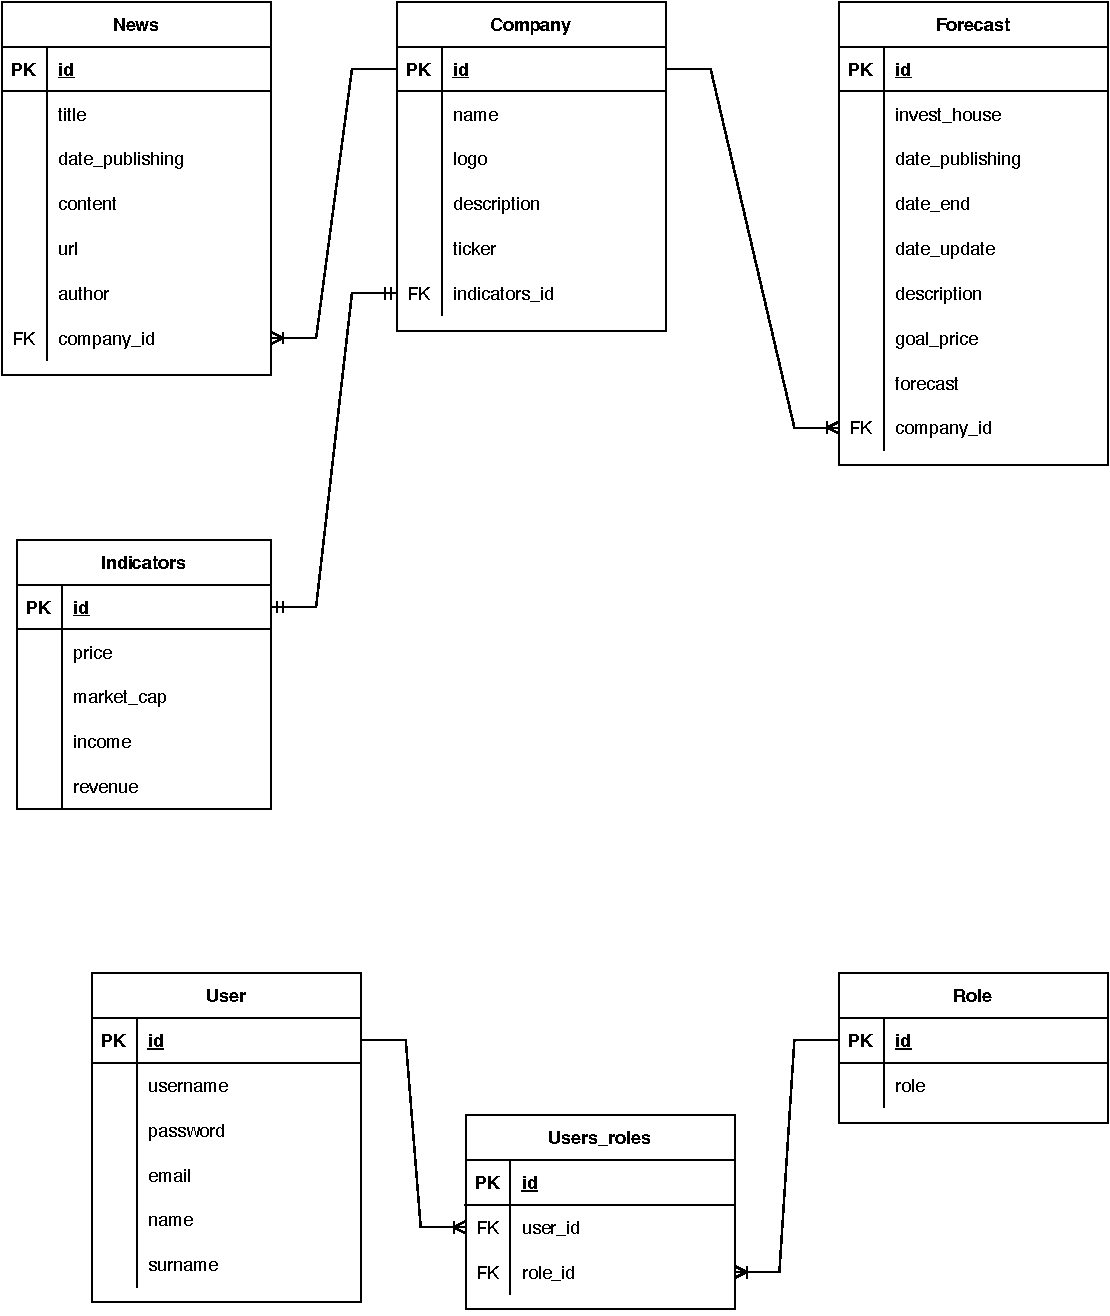
\includegraphics[scale=0.8]{img/database.pdf}
	\end{center}
	\captionsetup{justification=centering}
	\caption{Диаграмма спроектированной базы данных}
	\label{img:database}
\end{figure}

\newpage

Помимо этого, для всех таблиц будут реализованы триггеры, срабатывающие в момент удаления или обновления данных из таблиц. Данные триггеры служат для синхронизации данных в базе данных и в кэше.
\section{Проектирование базы данных кэширования}

База данных кэширования будет реализована с использованием Redis. Redis --- это нереляционная СУБД, хранящая данные в виде пар «ключ-значение».

В базе данных будут полностью продублированны таблицы из основной базы данных. Первичным ключом будет являться поле с уникальным идентификатором (\texttt{id}).
При повторном запросе данных у приложения сначала будет проводиться проверка, присутствует ли запись в кэше. В случае, если запись присутствует, запрос к основной базе данных производиться не будет и будут возвращены данные из кэша. В противном случае, будет произведен запрос к основной базе данных.

\section{Проектирование приложения}
Разрабатываемое приложение представляет собой многокомпонетное веб-приложение. Данные приложения будут получены с помощью REST API. Сервер обменивается данными с базами данных при помощи коннекторов, позволяющих делать запросы к базе данных с помощью  языка программирования. Схема архитектуры приложения представлена на рисунке \ref*{img:arch}.

\begin{figure}[h!]
	\begin{center}
		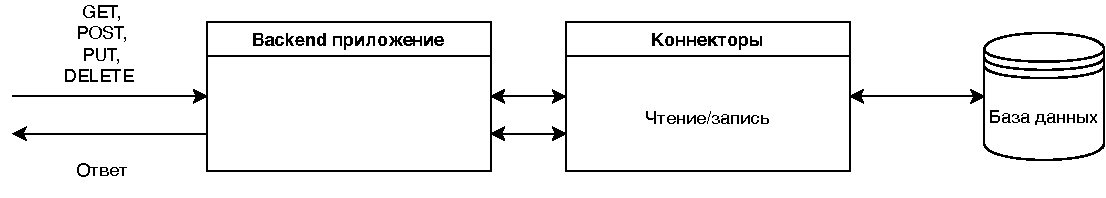
\includegraphics[scale=0.8]{img/architecture.pdf}
	\end{center}
	\captionsetup{justification=centering}
	\caption{Схема архитектуры спроектированного приложения}
	\label{img:arch}
\end{figure}

\section*{Вывод}

В данном разделе были представлены этапы проектирования баз данных и рассмотрена архитектура программного обеспечения.
